\documentclass{article} % For LaTeX2e
\usepackage{format/nips13submit_e}
\nipsfinalcopy % Uncomment for camera-ready version
\usepackage{times}
\usepackage{hyperref}
\usepackage[pdftex]{graphicx}
\usepackage{url}
\usepackage{color}
\usepackage{preamble}
\definecolor{mydarkblue}{rgb}{0,0.08,0.45}
\hypersetup{ %
    pdftitle={},
    pdfauthor={},
    pdfsubject={},
    pdfkeywords={},
    pdfborder=0 0 0,
    pdfpagemode=UseNone,
    colorlinks=true,
    linkcolor=mydarkblue,
    citecolor=mydarkblue,
    filecolor=mydarkblue,
    urlcolor=mydarkblue,
    pdfview=FitH}
    
    
\usepackage{graphicx, amsmath, amsfonts, bm, lipsum, capt-of}
\usepackage{natbib, xcolor, wrapfig, booktabs, multirow, caption}
\usepackage{float}

%\renewcommand{\baselinestretch}{0.99}

\def\ie{i.e.\ }
\def\eg{e.g.\ }

%\title{Automatic Summarization of Composite Nonparametric Time-Series Models}
\title{Automatic Construction and Natural-language Description of Additive Nonparametric Models}

\author{
James Robert Lloyd\\
University of Cambridge\\
%Department of Engineering\\
\texttt{jrl44@cam.ac.uk}
\And
David Duvenaud\\
University of Cambridge \\
%Department of Engineering \\
\texttt{dkd23@cam.ac.uk}
\And
Roger Grosse\\
M.I.T.\\
%Brain and Cognitive Sciences \\
\texttt{rgrosse@mit.edu}
\And
Joshua B. Tenenbaum\\
M.I.T.\\
%Brain and Cognitive Sciences \\
\texttt{jbt@mit.edu}
\And
Zoubin Ghahramani\\
University of Cambridge \\
%Department of Engineering \\
\texttt{zoubin@eng.cam.ac.uk}
}

\newcommand{\fix}{\marginpar{FIX}}
\newcommand{\new}{\marginpar{NEW}}

\setlength{\marginparwidth}{0.9in}
%%%%%%%%%%%%%%%%%%%%%%%%%%%%%%%%%%%%%%%%%%%%%%%%%%%%%%%%%%
%%%% EDITING HELPER FUNCTIONS  %%%%%%%%%%%%%%%%%%%%%%%%%%%
%%%%%%%%%%%%%%%%%%%%%%%%%%%%%%%%%%%%%%%%%%%%%%%%%%%%%%%%%%

%% NA: needs attention (rough writing whose correctness needs to be verified)
%% TBD: instructions for how to fix a gap ("Describe the propagation by ...")
%% PROBLEM: bug or missing crucial bit 

%% use \fXXX versions of these macros to put additional explanation into a footnote.  
%% The idea is that we don't want to interrupt the flow of the paper or make it 
%% impossible to read because there are a bunch of comments.

%% NA's (and TBDs, those less crucially) should be written so 
%% that they flow with the text.

\definecolor{WowColor}{rgb}{.75,0,.75}
\definecolor{SubtleColor}{rgb}{0,0,.50}

% inline
\newcommand{\NA}[1]{\textcolor{SubtleColor}{ {\tiny \bf ($\star$)} #1}}
\newcommand{\LATER}[1]{\textcolor{SubtleColor}{ {\tiny \bf ($\dagger$)} #1}}
\newcommand{\TBD}[1]{\textcolor{SubtleColor}{ {\tiny \bf (!)} #1}}
\newcommand{\PROBLEM}[1]{\textcolor{WowColor}{ {\bf (!!)} {\bf #1}}}

% as margin notes

\newcounter{margincounter}
\newcommand{\displaycounter}{{\arabic{margincounter}}}
\newcommand{\incdisplaycounter}{{\stepcounter{margincounter}\arabic{margincounter}}}

\newcommand{\fTBD}[1]{\textcolor{SubtleColor}{$\,^{(\incdisplaycounter)}$}\marginpar{\tiny\textcolor{SubtleColor}{ {\tiny $(\displaycounter)$} #1}}}

\newcommand{\fPROBLEM}[1]{\textcolor{WowColor}{$\,^{((\incdisplaycounter))}$}\marginpar{\tiny\textcolor{WowColor}{ {\bf $\mathbf{((\displaycounter))}$} {\bf #1}}}}

\newcommand{\fLATER}[1]{\textcolor{SubtleColor}{$\,^{(\incdisplaycounter\dagger)}$}\marginpar{\tiny\textcolor{SubtleColor}{ {\tiny $(\displaycounter\dagger)$} #1}}}


%% For submission, make all render blank.
%\renewcommand{\LATER}[1]{}
%\renewcommand{\fLATER}[1]{}
%\renewcommand{\TBD}[1]{}
%\renewcommand{\fTBD}[1]{}
%\renewcommand{\PROBLEM}[1]{}
%\renewcommand{\fPROBLEM}[1]{}
%\renewcommand{\NA}[1]{#1}  % Note, NA's pass through!

\begin{document}

\allowdisplaybreaks

\maketitle

\begin{abstract}
To complement a recently introduced automatic model-construction and search method, we demonstrate an automatic model-summarization procedure.
After automatically building an additive nonparametric regression model, our method constructs a report which visualizes and explains in words the meaning and relevance of each component.
These reports enable human model-checking and the understanding of complex modeling assumptions and structure.
We demonstrate this procedure on two time-series, showing that the automatically constructed models identify highly interpretable structures that can be automatically described in simple natural language.
\end{abstract}

\section{Introduction}
\vspace{-0.08in}

%Statistical modeling is often performed in an iterative manner:  First, a simple model is proposed.  Second, the practitioner checks the model fit, often by looking for structure that wasn't captured by the model.

Simple parametric regression models such as linear regression are usually easily interpretable, and have well-established methods for model-checking.
In constrast, non-parametric models may be reasonably viewed with suspicion by the non-expert, since their assumptions may be difficult to check, and their predictive implications difficult to explain.

%Advances in nonparametric and compositional modeling have allowed fully automatic model search and construction of complex, structured, nonparametric regression models \cite{DuvLloGroetal13}.
%These automatically-constructed models have been used for extrapolation without further human intevention, but for model-checking or dataset exploration, extrapolations alone are insufficient.  
%Fortunately, the generated models are sufficiently structured to capture human-interpretable features in a given dataset, and the compositional nature of this structure allows for simple translation into natural language.

Recently, a method for searching over a large class of structured nonparametric regression models \citep{DuvLloGroetal13} was demonstrated to decompose time series into highly interpretable additive components.
In this initial work the interpretability of the model was described post-hoc by the authors, explaining how the learned structure of the model corresponded to the patterns in the additive components.

We extend this work by demonstrating that the structure of the models searched over allows for the automatic natural-language description of patterns within a data set.
% \ie the interpretable models are automatically interpreted!
We have also expanded and improved the components used in the model-construction process to improve the expressivity and interpretability of the models.

This paper contains extracts of human-readable reports automatically generated by our procedure.
The automatically generated text descriptions of the components of the models clearly communicate interpretable features of the data.
%This paper demonstrates a procedure for automatically generating a human-readable report, examining and explaining the properties of a given nonparametric model on a given dataset.
The supplementary material to this paper is a pair of complete reports generated by our method.
%These reports summarize and describe datasets modeled by a Gaussian process with a complicated kernel.
%The different components of the kernel correspond to different features of the dataset, and the report discusses in detail the properties and significance of each component.
%Detailed descriptions of the model construction and summarization procedure are deferred to future publications.

%Section \ref{sec:gpss} gives an overview of the structure search method which produces the models that our procedure summarizes.  Section \ref{sec:method} describes our method for generating these reports, and section \ref{sec:example} examines in detail the report included in the supplementary material.


\section{Gaussian Process Structure Search}
\label{sec:gpss}
\vspace{-0.08in}

The family of models described by our procedure are Gaussian process (\gp{}) models \cite{rasmussen38gaussian}.
%
%\subsection{Gaussian process regression}
\gp{}s use a kernel to define the covariance between any two function values, $\outputVar, \outputVar'$ evaluated at two inputs, $\inputVar,\inputVar'$ \ie ${\textrm{Cov}(\outputVar, \outputVar') = \kernel(\inputVar,\inputVar')}$.
%The kernel determines which sorts of structures the model places most of its probability mass upon, and in effect determines the generalization properties of the model.
The kernel specifies which structures are likely under the \gp{} prior, which in turn determines the generalization properties of the model.

Different kernels can express a wide variety of covariance structures, such as local smoothness or periodicity.
New kernels can be constructed by taking the product of a set of base kernels to express richer structures, such as functions which are locally periodic, or heteroscedastic.

The Gaussian process structure search (GPSS) procedure \citep{DuvLloGroetal13} searches over sums and products of a set of simple base kernels to produce an appropriate model for a given data set.
To produce the reports exhibited in this paper we used 6 base kernels that represent the following structures: smooth functions ($\kSE$), periodic functions ($\kPer$), linear functions ($\kLin$), constant functions ($\kC$), changepoints ($\kCP$), and white noise ($\kWN$).


%When given a dataset

\section{Description of kernel compositions}
\vspace{-0.08in}

For a given dataset, the GPSS method produces a compound kernel composed of sums and products of the 6 base kernels.  In this section, we describe how the properties of \gp{} models allow us to reduce the task of english-language summarization into relatively simple subproblems.

\subsection{Taking advantage of distributivity}
\vspace{-0.08in}

By distributivity, we can convert any compound kernel expression into a sum of products of base kernels.
For example, when the first version of {\sc GPSS} \citep{DuvLloGroetal13} was applied to airline passenger data, the syntax of the learned kernel structure was
\begin{equation}
\kSE \times \big( \kLin + \kLin \times ( \kPer + \kSE ) \big) + \kWN
\end{equation}
which can be distributed into a sum of products
\begin{equation}
(\kSE \times \kLin) + (\kSE \times \kLin \times \kPer) + (\kSE \times \kLin) + \kWN.
\end{equation}

%\paragraph{Additivity}
If $f_1(x) \dist \gp{}(0, \kernel_1)$ and $f_2(x) \dist \gp{}(0, \kernel_2)$ then $f_1(x) + f_2(x) \dist \gp{}(0, \kernel_1 + \kernel_2)$.
Therefore, a sum of kernels can be described as a sum of independent functions.
%
Thus, if we can automatically describe any product of base kernels, we can exactly describe our model as a sum of these components.  Thus, we only need to produce a procedure for describing products of base kernels.

\subsection{Description of products of base kernels}
\vspace{-0.08in}

Since the individual additive components produced by the GPSS method are produced by an open-ended grammar, it is impossible to write a lookup table to handle every type of component that GPSS might produce.  


%\subsubsection{Stationary Kernels}

We now examine the properties of products of base kernels.  We'll show that each kernel we multiply by modifies the properties of the resulting prior on functions in a consistent way.  This means that, for most cases, multiplying by another base kernel means we can simply append a set of adjectives to the description of the resulting function.

\subsubsection{Multiplication by a Squared-Exp Kernel}
\vspace{-0.08in}

Multiplying by an $\kSE$ kernel means that the resulting prior over functions now varies smoothly.  The degree of smoothness depends on the lengthscale of the kernel.%  We describe a kernel that has been multiplied by a $\kSE$ as a function ``that varies smoothly with a characteristic lengthscale
%
A product of two $\kSE$ kernels is exactly equivalent to a single $\kSE$ with different parameters.  This means that multiplication by an $\kSE$ kernel is an idempotent operation.  

For example,
the kernel $\kSE \times \kPer$ gives rise to functions which are \emph{locally} periodic: they only approximately repeat.
If the input space is restricted to a grid with spacing equal to the period of the periodic kernel, then $\kSE \times \kPer = \kSE$.
We therefore see that the functional form of the periodicity varies like $\kSE$, giving rise to the local nature of the periodicity.
%This observation extends similarly to kernels of the form $\kSE \times \prod \kPer$.

%At a syntactic level, mutliplication by $\kSE$ is idempotent \ie $\kSE \times \kSE = \kSE$.

\subsubsection{Multiplication by a White Noise kernel}
\vspace{-0.08in}

For stationary kernels, $\kWN$ behaves like zero.  For example, $\kWN \times \kSE = \kWN \times \kPer = \kWN$.  Thus the product of white noise with any kernel is simply white noise.


\subsubsection{Multiplication by the constant kernel}
\vspace{-0.08in}

The constant kernel $\kC$ behaves like the identity: $\kC \times k = k$.

%We now only need to describe the base kernels and products of the form $\kSE \times \prod \kPer$.

\subsubsection{Multiplication by a periodic kernel}
\vspace{-0.08in}

Multiplication by a periodic kernel means that each $f(x)$ will only covary with points near $f(x + n \tau)$, where $n$ is an integer and $\tau$ is the period of the kernel.
%
%\paragraph{ Products of Periodic Kernels}
This property also applies to products of periodic kernels.
Suppose that ${f_1(x) \dist \gp{}(0, \kernel_1)}$ and ${f_2(x) \dist \gp{}(0, \kernel_2)}$.
Then
\begin{equation}
{\textrm{Cov} \left[f_1(x)f_2(x), f_1(x')f_2(x') \right] = k_1(x,x')k_2(x,x')}.
\end{equation}
Therefore $\kPer \times \kPer$ defines a prior on functions whose covariance is the same as the product of independent periodic functions.  However, note that a product of periodic functions drawn from \gp{} priors will not be distributed according to a \gp{}.

%\subsubsection{Example}

%\begin{quotation}
%``This component is approximately periodic with a period of 1.0 years and varying amplitude. Across periods the shape of this function varies very smoothly. The amplitude of the function increases approximately linearly. The shape of this function within each period has a typical lengthscale of 6.1 weeks.''
%\end{quotation}


%\subsubsection{Non-Stationary Kernels}

\subsubsection{Multiplication by linear and changepoint kernels}
\vspace{-0.08in}

The linear ($\kLin$) and changepoint ($\kCP$) kernels both have the form $k(x,x') = a(x)a(x')$.  We can interpret kernels of this form in the following way:
Suppose that $f(x) \dist \gp{}(0, \kernel)$ and $a : \mathcal{X} \to \mathcal{Y}$ is a known function.
Then $a(x)f(x) \dist \gp{}\left(0, a(x) k(x, x') a(x') \right)$.

For example, the linear kernel, $\kLin$, has the form $\kLin(x, x') = c(x-a)(x'-a)$.
Setting $a(x) = \sqrt{c}(x-a)$ we see that multiplying a kernel, $\kernel$, by the linear kernel is equivalent to multiplying $f(x) sim \gp{}(0, k)$ by a linear function.
Similarly, multiplying by a changepoint kernel is equivalent to multiplying a \gp{} by a sigmoid function.

This interpretation means that we can separately describe the properties of the model arising from multiplication with kernels of the form $k(x,x') = a(x)a(x')$.
%
For example, multiplying by a linear kernel means that the amplitude of the function grows linearly away from a central point.  Multiplication by two kernels impplies quadratic growth, etc.

Changepoints are expressed in a similar manner:  By multiplying our function by a sigmoid, we can modulate the condtribution of any given kernel to go to zero in certain regions.  This modulation can be expressed through language such as ``this component applies from 1700 to 1800''.

%The univariate envelopes can be arbitrary products of linear functions and sigmoids which can be simply described by their parameters.



%\paragraph{Base kernels}

%The priors induced by the base kernels are well understood, with simple descriptions of typical functions.

%\begin{table}[ht]
%\centering
%\begin{tabular}{c|cc}
%Kernel & Function type & Description \\
%\midrule
%$\kWN$ & White noise & Each $f(x)$ is \iid\\
%$\kC$ & Constant & Every $f(x)$ is identical \\
%$\kSE$ & Smooth & samples of $f(x)$ are infinitely differentiable \\
%$\kPer$ & Periodic & samples of $f(x)$ are smooth but repeat exactly every period\\
%$\kLin$ & Linear & $f(x)$ is a straight line \\
%$\kCP$ & Sigmoid & Allows different covariance in different parts of the input space \\
%\end{tabular}
%\label{table:base-kernels}
%\end{table}





%The GPSS method produces a composite kernel which can be distributed into a sum of products.
%A sum of kernels corresponds to a sum of functions allowing a
%A sum of kernels directly corresponds to a sum of functions which allows for the models produced by GPSS to be decomposed naturally into a sum of parts.

% One property of Gaussian process models is that a sum of kernels is equivalent to a sum of functions.  This means that the models produced by GPSS can typically be decomposed into a sum of parts.

%Each part of the kernel defines a covariance function, which in turn describes a prior probability distribution over functions.  Conditioned on the dataset, the covariance functions also define a 

%\paragraph{Example}


%  Hence the part of the procedure which summarizes the individual components must be flexible, and also must present enough information that users can see the meaning of each component themselves.  We summarize each component both in writing and in plots.
%
%For the written portion, a first paragraph reports the type of component found, and the meaning of all kernel parameters in that component.  
%The compositional nature of kernel structures produced by GPSS allows for simple translation of individual components.
%Each type of kernel in a product of kernels modifies the form of the posterior in a consistent way, preventing the need for an infinite lookup table of descriptions.
%Table \ref{table:descriptions} gives some examples of high level summaries of functions.
%Since the posterior distribution also depends on the data, our summarizer includes heuristics to describe the shape of the components being modeled, such as ``smooth'' or ``monotonically increasing''.

%\begin{table}[ht]
%\begin{tabular}{l|l}
%Kernel & Description \\
%\midrule
%$\kPer$ & An exactly periodic function \\
%$\kPer \times \kSE$ & An approximately periodic function \\
%$\kPer \times \kSE \times \kLin$ & An approximately periodic function with linearly varying amplitude \\
%$\kLin$ & A linear function \\
%$\kLin \times \kLin$ & A quadratic function \\
%$\kPer \times \kLin \times \kLin$ & An exactly periodic function with quadratically varying amplitude\\
%\end{tabular}
%\caption{A demonstration of how it is possible to write an open-ended summarizer.  Different kernel structures modify the overall statistical structure of each component in independent ways.}
%\label{table:descriptions}
%\end{table}



%This sum decomposed the regression function into three additive components and additive noise.
%The second component was described by the authors as periodic ($\kPer$) with linearly ($\kLin$) increasing amplitude.
%The corresponding automatically generated description is able to give a more nuanced description


\subsection{Summary}  
\vspace{-0.08in}
We have broken down the problem of describing arbitary compositions of kernels into two manageable parts.  First, we distribute the composite kernel into a sum of products.  Second, for each product of kernels, we describe the properties of products of kernels $\kSE$, $\kPer$, $\kC$ and $\kWN$, and then append descriptions of the properties of the modulating functions implied by products of $\kLin$ and $\kCP$.

\section{Automatic Report Generation}
\label{sec:method}
\vspace{-0.08in}

Our report generation procedure takes as its starting point a dataset and a composite kernel, which together define a joint posterior probability distribution over a sum of functions.
The procedure summarizes properties of this complex distribution to the user through a comprehensive report.
%
These reports are designed to be intelligible to non-experts, illustrating the assumptions made by the model, describing the model's posterior distribution, and most importantly, enabling model-checking.
%\subsection{Design goals}
%
%\begin{itemize}
%\item {\bf Intelligibility}
%The procedure was designed to produce reports intelligible to non-experts.  
%
%\item {\bf Illustrate Model Assumptions}
%One of the main design criteria when designing our procedure was to make clear what assumptions the model is making, and what these assumptions imply in terms of extrapolation.  Even when simple Gaussian process models are used, it is often unclear what structure was captured by the model and what was not.
%
%\item {\bf Illustrate Posterior Uncertainty}
%One of the selling points of Bayesian modeling over point estimates is that they produce a rich posterior distribution over possible explanations of the data.  However, this posterior distribution is often quite a complex object, and is usually difficult to summarize.
%
%\item {\bf Enable Model-checking}
%One of the most important reasons to examine a model is to discover flawed assumptions, or structure not captured by the model.  Simply examining residuals, cross-validation or marginal likelihood scores is often not sufficient to notice when the model is failing to capture.
%\end{itemize}
%
%\subsection{Report structure}

These reports have three sections: an executive summary, a detailed discussion of each component, and a section discussing how the model extrapolates beyond the range of the data.

\begin{itemize}
\item { \bf Executive Summary} The first section of each report describes which structures were discovered in the model, and the relative importance of the different components in explaining the data.
\item { \bf Decomposition plots}
The second section of each report contains a detailed discussion of each component.
Every component is plotted, and properties of the covariance structure are described.
%Some components are not meaningful when plotted on their own, so we also include plots of the cumulative sum of components.
%\paragraph{Automatic Plotting}
Each component's posterior is plotted in two ways.  First, the posterior mean and variance of each component is plotted on its own.  Second, the posterior mean and variance of all components shown so far is plotted against the data.  This progression of plots 
%By contrasting each of these plots with plots of earlier components, we can see 
shows qualitatively how each component contributes to an overall explanation of the data.
%A second paragraph explains the improvement in predictive performance gained by including this component in the model. This is the same information as included in the executive summary.
\item {\bf Extrapolation plots}
The third section of each report shows extrapolations into the future, as well as posterior samples from each individual component of the model.  These samples help to characterize the uncertainty expressed by the model, and the extent to which different components contribute to predicting the future behavior of a time series.
%
The predictive mean and variance of the signals shown in the summary plots are useful, but do not capture the joint correlation structure in the posterior.  Showing posterior samples is a simple and universal way to illustrate joint statistical structure.
\end{itemize}

An additional section that automatically describes model-checking procedures is work in progress.

%\vspace{-0.05in}

\subsection{Example: Summarizing 400 Years of Solar Activity}
\label{sec:example}
\vspace{-0.1in}

To give an example of the capabilities of our procedure, we show excerpts from the report automatically generated on annual solar irradiation data from 1610 to 2011.  This time series has two obvious features: a roughly 11-year cycle of solar activity, and a period lasting from 1645 to 1715 with much smaller variance than the rest of the dataset.  This flat region corresponds to the Maunder minimum, a period in which sunspots were extremely rare \citep{lean1995reconstruction}.
%
The GPSS search procedure and automatic summary clearly identify these two features, as discussed below.



\begin{figure}[h!]
\centering
\fbox{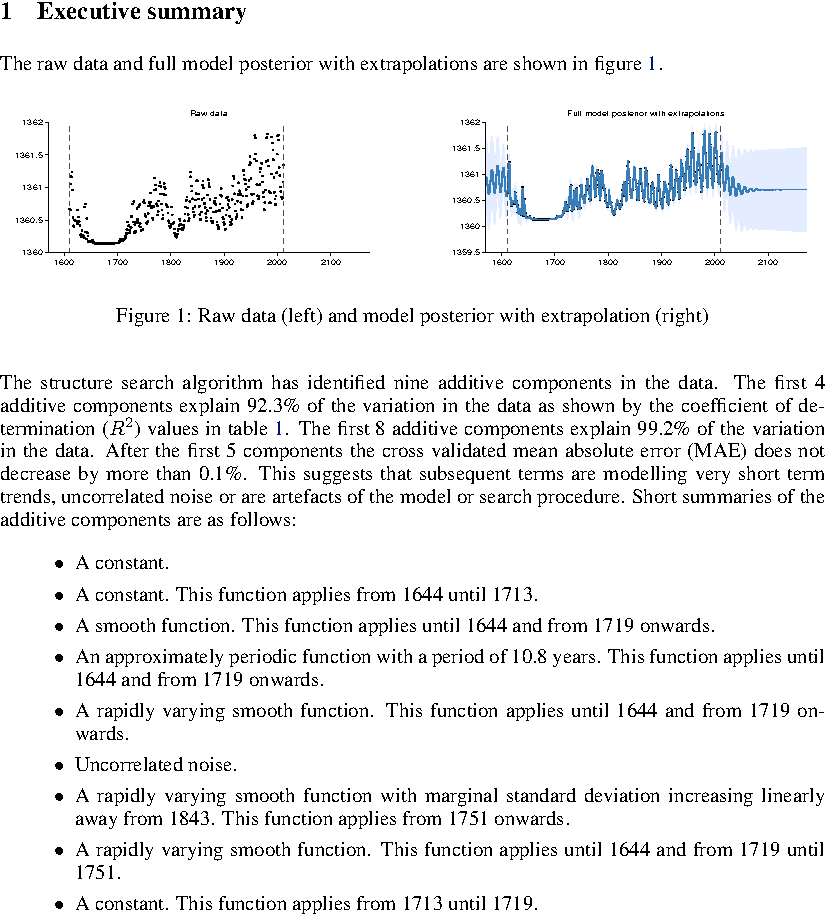
\includegraphics[trim=0cm 3.4cm 0cm 6.3cm, clip, width=0.98\columnwidth]{solarpages/02-solar-seperate-pages-2}}
\caption{
An example of an automatically-generated summary of a dataset.  The dataset is decomposed into diverse types of structures, and each structure is explained in simple terms.}
\label{fig:exec}
\end{figure}


Figure \ref{fig:exec} shows the automatically-generated summary of the solar dataset.
The model uses 9 additive components to explain the data, and reports that the first 4 components explain more than 90\% of the variance in the data.
%This might seem incongruous with the observation that there are two main features of the data, but if we examine the first four components, we see that the first component is describing the mean of the dataset, the second is the Maunder minimum, the third describes the long-term trend, and the fourth describes the 11-year periodicity.
Just from the short summaries of the additive components we can see that the model has identified the Maunder minimum (second component) and 11-year solar cycle (fourth component).
%This might seem incongruous with the observation that there are two main features of the data, but if we examine the first four components, we see that the first component is describing the mean of the dataset, the second is the Maunder minimum, the third describes the long-term trend, and the fourth describes the 11-year periodicity.

%\subsubsection{Signal versus Noise}
%
%One design challenge we encountered was seperating the recovered structure into signal and noise.  Originally, the model always included a term corresponding to \iid{} additive Gaussian noise.  However, in practice, the distinction between signal and noise is unclear for two reasons.  First, a component which varies arbitrarily quickly in time can be indistinguishable from noise.  Second, the variance of the noise may change over time (called heteroskedasticity), and this sort of pattern may be considered part of the signal.
%Because of the blurry distinction between signal and noise, we include a table which summarizes the relative contribution of each component in terms of held-out predictive power.%  To do this, we order the components in terms of how much each one improves predictive performance in a 10-fold cross-validation procedure.  The intuition for this metric is that noise-like components do not contribute much to the extrapolation performance of the model, but that signal-like components do.
%
%
%\begin{figure}
%\centering
%\fbox{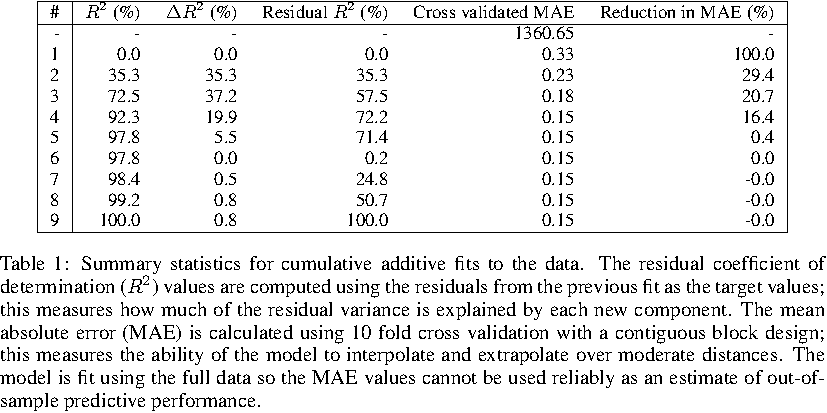
\includegraphics[width=0.98\columnwidth]{solarpages/02-solar-seperate-pages-3}}
%\caption{A table summarizing the relative contribution of the 9 different components of the model in terms of predictive performance.}
%\label{fig:table}
%\end{figure}
%
%Figure \ref{fig:table} show an example of this table on the solar dataset.

%Because the user may be interested in local or noisy components, we report all components to the user.  
%An interactive version of our procedure could allow users to specify which components are of interest, and group the remaining components into a single noise component.




\begin{figure}[h!]
\centering
\fbox{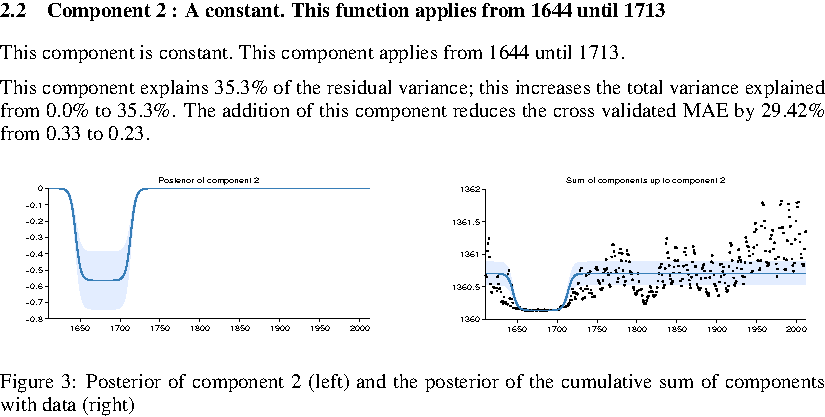
\includegraphics[trim=0cm 0cm 0cm 0.7cm, clip, width=0.98\columnwidth]{solarpages/02-solar-seperate-pages-5}}
\caption{Discovering the Maunder minimum.  The kernel found by GPSS contained a pair of changepoints bracketing the period of low solar activity.}
\label{fig:maunder}
\end{figure}

% is a good example of a meaningful component discovered by GPSS, whose meaning would be unclear without an individual plot.  


%In the history of solar activity, the Maunder minimum is a good example of a local change in covariance.  Specifically, 
%The changepoint kernels used by GPSS encode changes in covariance structure.
%For example, from about 1645 to 1715, solar activity decreased.
%, and very few sunspots were observed, a period called the Maunder Minimum \citep{lean1995reconstruction}.
Figure \ref{fig:maunder} shows that GPSS has captured the unusual period of decreased solar activity from about 1645 to 1715 and is able to report this in natural language.
This feature was captured by the model by multiplying a constant kernel by two changepoint kernels.
Figure \ref{fig:periodic} shows that GPSS has isolated the approximately 11 year solar cycle.
%with a pair of changepoint kernels.%shows exactly which sort of structure was recovered by this component.

%\begin{figure}[h!]
%\centering
%\fbox{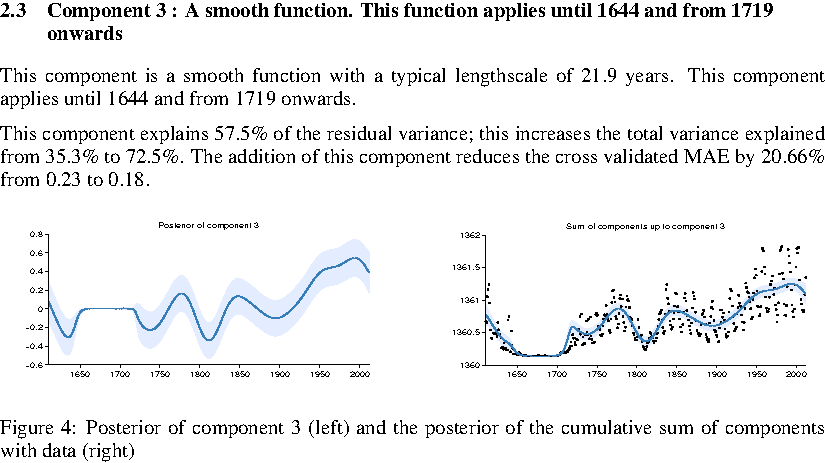
\includegraphics[width=0.98\columnwidth]{solarpages/02-solar-seperate-pages-6}}
%\caption{Characterizing the medium-term smoothness of solar activity levels.  By allowing other components to explain the periodicity, noise, and the Maunder minimum, we can isolate the part of the signal best explained by a slowly-varying trend.}
%\label{fig:smooth}
%\end{figure}

%\paragraph{Isolating the smoothly-varying component} Examining the dataset by eye, overall solar activity seems to change slowly over decades.  However, this intuition seems difficult to formalize.  Linear or quadratic regression is clearly inappropriate, and methods based on local smoothing would need to control for the periodic component.  Luckily, the GPSS procedure does exactly this, allowing us to isolate the slowly-varying component of the data, without having to forecast either the Maunder minimum or the periodic variation.  Figure \ref{fig:smooth} shows the automatically-generated summary of this component.

\begin{figure}[h!]
\centering
\fbox{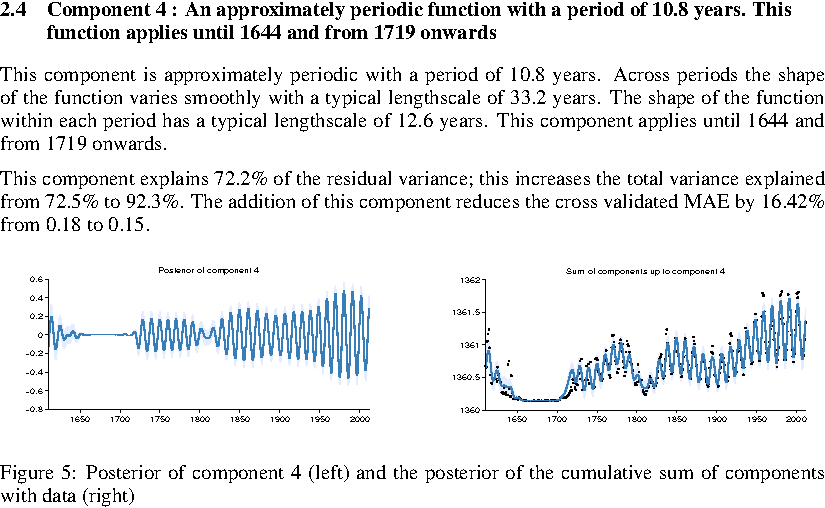
\includegraphics[trim=0cm 0cm 0cm 4.7cm, clip, width=0.98\columnwidth]{solarpages/02-solar-seperate-pages-7}}
\caption{Isolating the periodic component of the dataset.  By isolating this aspect of the statistical structure, we can easily observe additional features, such as the shape of the peaks and troughs, or the fact that the amplitude changes over time.}
\label{fig:periodic}
\end{figure}

%Figure \ref{fig:periodic} shows that GPSS has identified the approximately 11 year solar cycle.
%By isolating this component in separate plots it is easy to see the exact nature of the solar cycle \eg how the amplitude of this periodic component varies over time.
%This demonstrates one benefit of isolating individual components: we can now see, by eye, extra structure that was not explicitly captured by the model.  Specifically, we can see that the amplitude of the periodic component varies over time.

%and by comparing with figure \ref{fig:smooth}, we can see that it varies roughly in proportion to the overall magnitude of the signal.
%  This pattern suggests that some sort of log-transform might be appropriate for this dataset, or that the model should be extended in some way to capture this structure.


%
\begin{figure}[ht]
\centering
\fbox{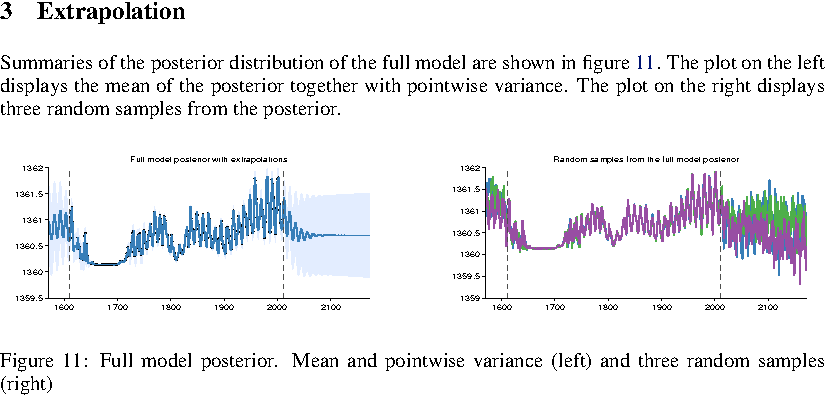
\includegraphics[trim=0cm 0cm 0cm 2.8cm, clip, width=0.98\columnwidth]{solarpages/02-solar-seperate-pages-13}}
\caption{Sampling from the posterior.  These samples help show not just the predictive mean and variance, but also the predictive covariance structure.  Note, for example, that the predictive mean (left) does not exhibit periodicity, but the samples (right) do.}
\label{fig:extrap-full}
\end{figure}
%
%For example,
%  shows the predictive mean and variance given the entire model. 
It is not clear from the left-hand plot in figure \ref{fig:extrap-full} whether or not the periodicity of the dataset is expected to continue into the future.  However, from the samples on the right-hand size, we can see that this is indeed the case.  

%\begin{figure}[h!]
%\centering
%\fbox{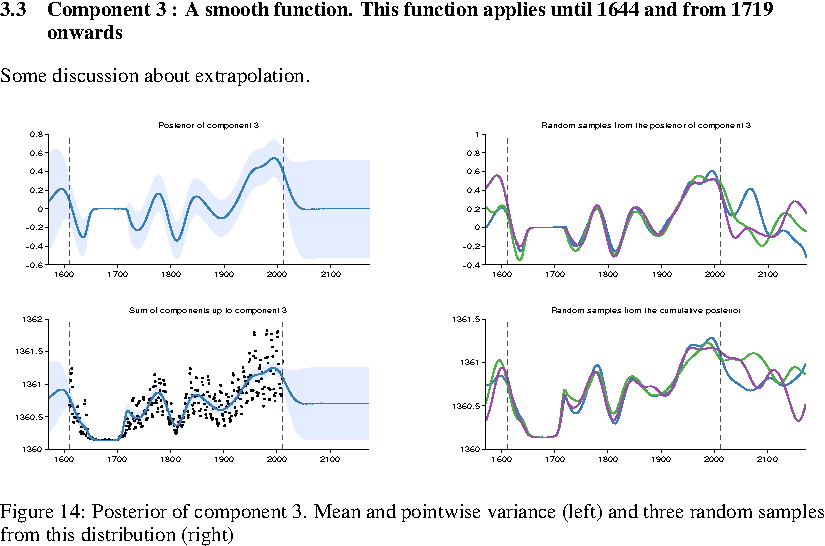
\includegraphics[width=0.98\columnwidth]{solarpages/02-solar-seperate-pages-16}}
%\caption{Extrapolating a single component of the model.  Because our model class allows us to isolate individual components, we can show the extent to which the model expects different trends to continue.  We also observe that the posterior samples are quite different from the posterior mean, away from the data.}
%\label{fig:extrap-smooth}
%\end{figure}

%\paragraph{Extrapolating individual components}
%We can also examine the model's expectations about the future behavior of individual components through sampling.  Further plots in the extrapolation section show posterior samples for each individual additive component. %For example, in figure \ref{fig:extrap-smooth}, we are shown samples of the predictive distribution of the smooth component of variation.  This plot indicates that the model considers a wide range of future average intensities to be plausible, but that it always expects those average intensities to vary smoothly.

%\section{Related Work}

%There exists a vast literature on both model visualization and model checking.


%\paragraph{Structure learning in Bayesian networks}
%Similar idea of discovering semantics via model search.
%Semantics are more vague though \ie a probability table is not an entirely concise summary

%\paragraph{Linear model}
%These discover highly interpretable semantics but are limited in expressivity

%\paragraph{Nonparametric additive models}
%Highly flexible but semantics are vague \ie can only talk about smooth functions

%\paragraph{Equation learning}
%Very flexible but semantics of equations do not map onto human understanding \eg saw tooth vs Fourier decomposition of a saw tooth - which is more human understandable?
%How would you explain a sensor error with Eureqa style equations.

%\paragraph{Deep learning}
%Again very flexible but the semantics are not usually human interpretable.
%How can we understand the output of complex representation learning algorithms without human intervention (\eg recognising that your deep net has become a cat classifier).

%\paragraph{Kernel search}
%Can use the precise semantics of linear models or the vague semantics of nonparametric additive models and other components along this spectrum.
%Flexible modelling with components that a human might use to describe what is going on.


\paragraph{Source Code}
Python code to perform all experiments is available on github.\footnote{Available at 
\href{http://www.github.com/jamesrobertlloyd/gpss-research}
{\texttt{github.com/jamesrobertlloyd/gpss-research}}}
%All \gp{} hyperparameter tuning was performed by automated calls to the GPML toolbox\footnote{Available at 
%\href{http://www.gaussianprocess.org/gpml/code/}
%{\texttt{www.gaussianprocess.org/gpml/code/}}
%}

%\section{Discussion and Future Work}

%\begin{quotation}
%``The availability of 'user-friendly' statistical software has caused authors to become increasingly careless about the logic of interpreting their results, and to rely uncritically on computer output, often using the 'default option' when something a little different (usually, but not always, a little more complicated) is correct, or at least more appropriate.''
% In trying to practice this art, the Bayesian has the advantage because his formal apparatus already developed gives him a clearer picture of what to expect, and therefore a sharper perception for recognizing the unexpected.

%\defcitealias{dyke1997avoid}{G. Dyke, 1997}
%\hspace*{\fill}\citet{Jaynes85highlyinformative}
%\hspace*{\fill}\citetalias{dyke1997avoid}
%\end{quotation}

%In this paper, we exhibited the output of a method for automatically constructing and summarizing a compositional Gaussian process regression model in natural language.
%These summaries can enable human experts and non-experts to understand the implications of a model, check its plausibility, and notice structure not yet captured by the model.

%\pagebreak

\bibliographystyle{unsrt}
\bibliography{gpss}

\end{document}
